\documentclass[tikz,border=8pt]{standalone}
\usepackage{tikz}
\definecolor{bg}{HTML}{171D2B}
\definecolor{ak}{HTML}{F7B538}
\definecolor{tx}{HTML}{F1F5F9}
\definecolor{mu}{HTML}{94A3B8}
\begin{document}
\pagecolor{bg}
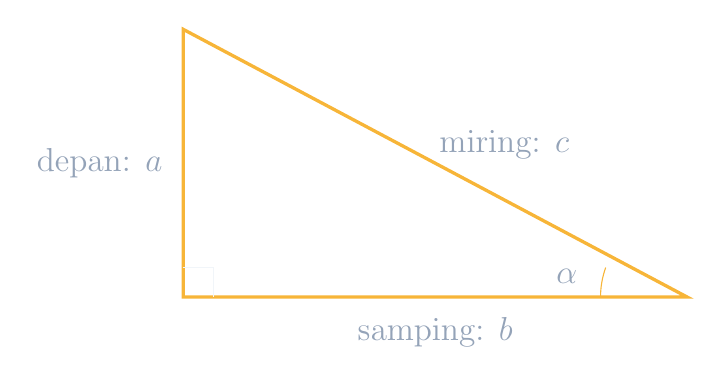
\begin{tikzpicture}[>=stealth, text=tx, font=\large]
  % triangle: right angle at C(0,0), A(0,3.4), B(6.4,0)
  \coordinate (C) at (0,0);
  \coordinate (A) at (0,3.4);
  \coordinate (B) at (6.4,0);
  \draw[very thick, ak] (A) -- (B) -- (C) -- cycle;
  \draw[tx] (0,0.38) -- (0.38,0.38) -- (0.38,0);
  % angle alpha arc at B
  \draw[ak, thin] ([shift=(160.06:1.1)]B) arc[start angle=160.06, end angle=180, radius=1.1];
  \node[mu] at ([shift=(170:1.55)]B) {$\alpha$};
  % side labels
  \node[mu, left=4pt] at (0,1.7) {depan: $a$};
  \node[mu, below=4pt] at (3.2,0) {samping: $b$};
  \node[mu, above right=-2pt] at (3.2,1.7) {miring: $c$};
\end{tikzpicture}
\end{document}
